\chapterimage{orange2.jpg} % Chapter heading image
\chapterspaceabove{6.75cm} % Whitespace from the top of the page to the chapter title on chapter pages
\chapterspacebelow{7.25cm} % Amount of vertical whitespace from the top margin to the start of the text on chapter pages

\chapter{Input-Output Stability}\index{Input-Output Stability}

\section{Overview}\index{Overview}

So far, stability was studied using Lyapunov functions focusing on internal states. Input-Output (I/O) Stability, in contrast, studies how bounded inputs produce bounded outputs using the mapping $y = H(u)$. It treats the system as a black box without considering internal states.  

\begin{center}
\begin{tikzpicture}[auto, node distance=1.5cm, thick]
  \node (u) {$u(t)$};
  \node[draw, rectangle, minimum height=1.5cm, minimum width=2.5cm, right=of u] (H) {$H$};
  \node (y) [right=of H] {$y(t)$};
  \draw[->] (u) -- (H);
  \draw[->] (H) -- (y);
\end{tikzpicture}
\end{center}

\section{Function Spaces}\index{Function Spaces}

So far we studied vector spaces of finite-dimensional vectors.  
Now we study \textbf{function spaces}, where the elements are \emph{functions} instead of vectors.  

\begin{definition}[Function space]
A \emph{function space} is a set of functions from a domain (e.g.\ time, $\mathbb{R}_{\geq 0}$) into a codomain (e.g.\ $\mathbb{R}^q$) that is equipped with additional structure, such as operations (addition, scalar multiplication) and possibly a norm or inner product.  
For example, we may consider
\[
u:\mathbb{R}_{\geq 0} \to \mathbb{R}^q, 
\quad 
u(t) =
\begin{bmatrix}
u_1(t) \\ \vdots \\ u_q(t)
\end{bmatrix}.
\]
\end{definition}

\subsection{$L_p$ Spaces}

A particularly important class of function spaces in analysis and control are the $L_p$ spaces.

\begin{definition}[$L_p$ space]
For $1 \leq p < \infty$, the space $L_p(0,\infty;\mathbb{R}^q)$ is defined as
\[
L_p = \Big\{ u:\mathbb{R}_{\geq 0}\to \mathbb{R}^q \;\Big|\;
\int_{0}^{\infty} \|u(t)\|^p \, dt < \infty \Big\}.
\]
The corresponding norm is
\[
\|u\|_{L_p} = \left( \int_{0}^{\infty} \|u(t)\|^p \, dt \right)^{1/p}.
\]
\end{definition}

\begin{definition}[$L_2$ space]
The \emph{square-integrable space} is the case $p=2$:
\[
L_2(0,\infty;\mathbb{R}^q) 
= \Big\{ u:\mathbb{R}_{\geq 0}\to \mathbb{R}^q \;\Big|\;
\int_{0}^{\infty} \|u(t)\|^2 \, dt < \infty \Big\}.
\]
The norm
\[
\|u\|_{L_2} = \left( \int_{0}^{\infty} \|u(t)\|^2 \, dt \right)^{1/2}
\]
represents the \textbf{energy} of the signal.
\end{definition}

\begin{definition}[$L_\infty$ space]
The \emph{essentially bounded space} is defined as
\[
L_\infty(0,\infty;\mathbb{R}^q) 
= \Big\{ u:\mathbb{R}_{\geq 0}\to \mathbb{R}^q \;\Big|\;
\sup_{t \geq 0} \|u(t)\| < \infty \Big\}.
\]
The norm
\[
\|u\|_{L_\infty} = \sup_{t \geq 0} \|u(t)\|
\]
represents the \textbf{maximum amplitude} of the signal.
\end{definition}

\begin{remark}
\begin{itemize}
\item  $L_2$ is widely used to measure signal energy (that's why used in stability analysis).  
\item  $L_\infty$ is used to measure boundedness or peak values of signals.  
\item  In general, $L_p$ spaces allow us to study signals with different growth and smoothness properties, and they provide the foundation for many results in control and signal processing.
\end{itemize}
\end{remark}

\begin{proposition}[Hölder’s inequality]
Let $p,q > 1$ with $\tfrac{1}{p}+\tfrac{1}{q}=1$.  
If $f \in L_p(0,T)$ and $g \in L_q(0,T)$, then $fg \in L_1(0,T)$ and 
\[
\int_{0}^{T} |f(t)g(t)| \, dt 
\;\leq\;
\left( \int_{0}^{T} |f(t)|^p \, dt \right)^{1/p}
\left( \int_{0}^{T} |g(t)|^q \, dt \right)^{1/q}.
\]
\end{proposition}

\begin{proposition}[Minkowski’s inequality]
For $1 \leq p < \infty$, if $f,g \in L_p(0,T)$, then
\[
\|f+g\|_{L_p} \;\leq\; \|f\|_{L_p} + \|g\|_{L_p}.
\]
Thus $\|\cdot\|_{L_p}$ defines a norm on $L_p$.
\end{proposition}

\subsection{Extended Spaces}\index{Function Spaces!Extended}

\begin{definition}[Truncation operator]
Let $X$ be a function space on $[0,\infty)$.  
For $T>0$, the \emph{truncation operator} $P_T:X \to X$ is defined by
\[
(P_Tu)(t) =
\begin{cases}
u(t), & 0 \leq t \leq T,\\[6pt]
0, & t > T.
\end{cases}
\]
\end{definition}

\begin{definition}[Extended space]
Let $X$ be a function space on $[0,\infty)$.  
The \emph{extended space} $X_e$ is defined as
\[
X_e = \big\{ u:[0,\infty)\to\mathbb{R}^q \;\big|\; 
P_T u \in X \;\; \text{for all } T>0 \big\}.
\]
In words: $u \in X_e$ if \textbf{every finite-time truncation} of $u$ belongs to $X$.
\end{definition}

\begin{example}
If $X = L_2(0,\infty)$, then
\[
X_e = \{ u:[0,\infty)\to \mathbb{R}^q \mid u \in L_2(0,T) \;\;\forall T>0\}.
\]
Thus $X_e$ contains all signals that have \textbf{finite energy on every bounded interval}, even if their total energy on $[0,\infty)$ is infinite.  
For example, $u(t)=1$ is not in $L_2(0,\infty)$, but $u \in (L_2)_e$ since its truncation to any finite interval lies in $L_2(0,T)$.
\end{example}

\begin{remark}
The extended space $X_e$ enlarges $X$ by admitting signals that are locally in $X$ but not globally.  
This is useful in control theory because real signals are often studied over finite horizons.
\end{remark}

\section{Input-Output Stability}\index{Input-Output Stability}

\begin{definition}[Mapping]
The mathematical representation of a physical system is defined as a mapping
\[
H: X_e \to X_e
\]
that satisfies the \textbf{causality condition}:
\[
(Hu)_T = \big(H(u_T)\big)_T, \qquad \forall u \in X_e, \; T>0,
\]
where $X_e$ is the space consisting of all functions whose truncation belongs to $X$.
\end{definition}

\begin{example}
Consider the first-order causal system:
\[
\dot{y}(t) + y(t) = u(t), \qquad y(0) = 0.
\]

Let the input $u(t)$ be a step function. Its truncated version at $T=4$ is denoted $u_T(t)$. Then the system outputs satisfy the causality condition:
\[
(Hu)_T = (H(u_T))_T.
\]

\begin{center}
\begin{tikzpicture}[auto, node distance=1.5cm, thick]
  % First: full input
  \node (u) {$u(t)$};
  \node[draw, rectangle, minimum height=1.5cm, minimum width=2.5cm, right=of u] (H) {$H$};
  \node (y) [right=of H] {$(Hu)(t)$};
  \draw[->] (u) -- (H);
  \draw[->] (H) -- (y);
\end{tikzpicture}

\vspace{1cm}

\begin{tikzpicture}[auto, node distance=1.5cm, thick]
  % Second: truncated input
  \node (uT) {$u_T(t)$};
  \node[draw, rectangle, minimum height=1.5cm, minimum width=2.5cm, right=of uT] (H) {$H$};
  \node (yT) [right=of H] {$(H(u_T))(t)$};
  \draw[->] (uT) -- (H);
  \draw[->] (H) -- (yT);
\end{tikzpicture}
\end{center}

\begin{center}
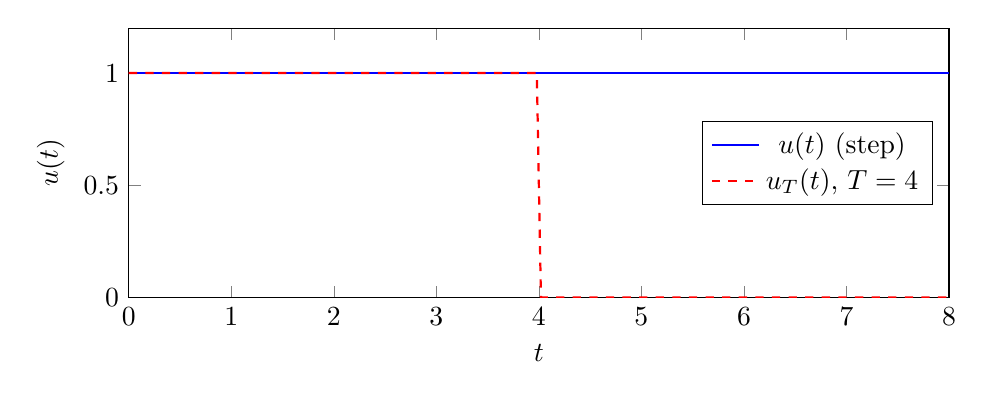
\begin{tikzpicture}
\begin{axis}[
    width=12cm, height=5cm,
    xlabel={$t$}, ylabel={$u(t)$},
    xmin=0, xmax=8, ymin=0, ymax=1.2,
    samples=200, domain=0:8,
    legend style={at={(0.98,0.5)},anchor=east}
]
\addplot[blue, thick] {x>=0 ? 1 : 0}; 
\addlegendentry{$u(t)$ (step)}

\addplot[red, dashed, thick] {x<=4 ? 1 : 0}; 
\addlegendentry{$u_T(t)$, $T=4$}
\end{axis}
\end{tikzpicture}

\vspace{0.5cm}

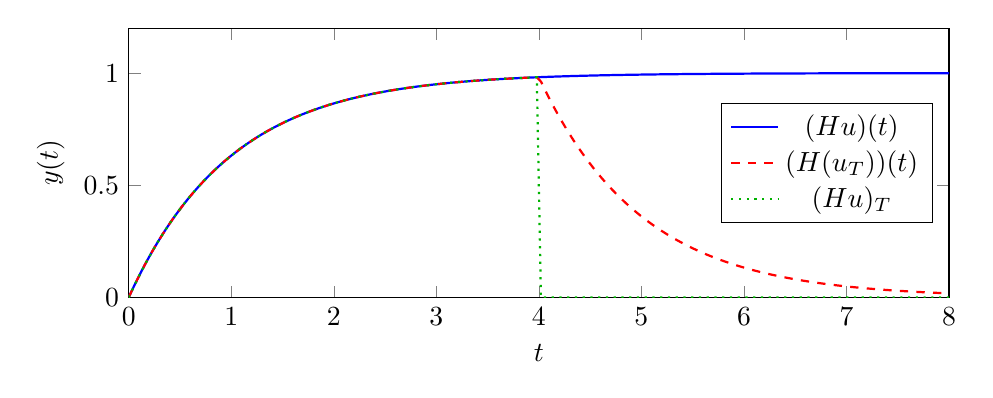
\begin{tikzpicture}
\begin{axis}[
    width=12cm, height=5cm,
    xlabel={$t$}, ylabel={$y(t)$},
    xmin=0, xmax=8, ymin=0, ymax=1.2,
    legend style={at={(0.98,0.5)},anchor=east}
]
% Full system response
\addplot[blue, thick, samples=200, domain=0:8] {1 - exp(-x)};
\addlegendentry{$(Hu)(t)$}

% Truncated input system response
\addplot[red, dashed, thick, samples=200, domain=0:8] {x<=4 ? (1 - exp(-x)) : (1 - exp(-4))*exp(-(x-4))};
\addlegendentry{$(H(u_T))(t)$}

% Output truncation
\addplot[green!70!black, dotted, thick, samples=200, domain=0:8] {x<=4 ? (1 - exp(-x)) : 0};
\addlegendentry{$(Hu)_T$}
\end{axis}
\end{tikzpicture}
\end{center}
\end{example}

\begin{remark}
For a causal system, the output at any time $t$ depends only on the input values up to that time. Therefore, if we truncate the input at time $T$ to obtain $u_T(t)$, the resulting output $(H(u_T))(t)$ matches the original output $(Hu)(t)$ for all $t \le T$. Moreover, truncating the original output at $T$, i.e., $(Hu)_T$, gives exactly the same signal. This property formally captures the essence of input-output causality.
\end{remark}

\begin{definition}[Finite-Gain System]
A system $H$ is said to have a \textbf{finite gain} if there exist constants 
\(\gamma(H) < \infty\) (called the \emph{gain} of $H$) and \(\beta \in \mathbb{R}^+\) such that, for all inputs \(u \in X_e\),
\[
\| Hu \|_X \le \gamma(H) \, \| u \|_X + \beta.
\]

Here, \(\beta\) is a bias term which may be nonzero even when \(u = 0\).  
If \((Hu) = 0\) whenever \(u = 0\), then \(\beta = 0\), and the gain can be calculated as
\[
\gamma(H) = \sup_{u \neq 0} \frac{\| (Hu)_T \|_X}{\| u_T \|_X}.
\]
\end{definition}

\begin{example}[First-Order Linear System]
Consider the system
\[
\dot{y}(t) + y(t) = u(t), \quad y(0)=0,
\]
with input \(u(t) \in L_\infty[0,\infty)\).  

- The output is 
\[
y(t) = \int_0^t e^{-(t-\tau)} u(\tau) \, d\tau.
\]  

- Using the norm \(\| \cdot \|_\infty\), we can estimate
\[
|y(t)| \le \int_0^t e^{-(t-\tau)} |u(\tau)| \, d\tau \le \| u \|_\infty \int_0^t e^{-(t-\tau)} d\tau \le \| u \|_\infty.
\]

Thus, the system has \textbf{finite gain} with 
\[
\gamma(H) = 1, \quad \beta = 0.
\]
\end{example}

\section{LTI Systems}\index{LTI Systems}

We study Linear Time-Invariant (LTI) systems in terms of input-output behavior instead of state-space models, focusing on SISO systems for simplicity.  

%------------------------------------------------
\begin{definition}[Set $A$]  
A function $f$ belongs to the set $\mathcal{A}$ if
\[
f(t) = f_0\delta(t) + f_a(t), \quad t \geq 0,
\]
and $f(t) = 0$ for $t < 0$, where
\[
f_a \in L_1, \quad \int_0^\infty |f_a(\tau)| \, d\tau < \infty.
\]
The norm is defined as
\[
\|f_a\| = f_0 + \int_0^\infty f_a(t)\, dt.
\]
\end{definition}

\begin{definition}[Laplace Transform Set]  
Let $\hat{\mathcal{A}}$ be the set of Laplace transforms of $A$. That is,
\[
\hat{\mathcal{A}} = \{ F(s) = \mathcal{L}\{f(t)\} \mid f \in A \}.
\]
\end{definition}

\begin{definition}[Proper and Strictly Proper Rational Functions]  
Let $\mathbb{R}[s]$ denote the set of polynomials in $s$, and $\mathbb{R}(s)$ the field of fractions of $\mathbb{R}[s]$.  

A rational function $\hat{M}(s) \in \mathbb{R}(s)$ is called:  
\begin{itemize}
    \item \textbf{Proper} if $\displaystyle \lim_{s \to \infty} \hat{M}(s) < \infty$; equivalently, the degree of the numerator is less than or equal to the degree of the denominator in the Laplace domain.
    \item \textbf{Strictly Proper} if $\displaystyle \lim_{s \to \infty} \hat{M}(s) = 0$; equivalently, the degree of the numerator is strictly less than that of the denominator in the Laplace domain.
\end{itemize}
According to this, $H^\cap(s)$ (Laplace transform of the impulse response) is strictly proper.
\end{definition}

\begin{theorem}  
If $\hat{F}(s) \in \mathbb{R}(s)$, then $F(s) \in \hat{\mathcal{A}}$ if and only if:
\begin{enumerate}
    \item $F^\cap(s)$ is proper, and  
    \item All poles of $F^\cap(s)$ lie in the left-half plane.  
\end{enumerate}
\end{theorem}

\begin{definition}[Convolution]  
For functions $f$ and $g$, their convolution is defined as
\[
(f * g)(t) = \int_0^t f(\tau) g(t-\tau)\, d\tau.
\]
\end{definition}

\begin{definition}[Convolution Operator]  
An LTI system $H$ is a convolution operator if
\[
H(u(t)) = (h * u)(t),
\]
where $h(\cdot)$ is called the \textbf{kernel} (impulse response) of $H$.  
\end{definition}

\begin{theorem}[Lp Stability]  
Consider an LTI system $H$ with impulse response
\[
h(t) = h_0 \delta(t) + h_a(t).
\]  
Then $H$ is $L_p$ stable if and only if $h \in A$, and moreover
\[
\|Hu\|_{L_p} \;\leq\; \|h\|_{L_p}\, \|u\|_{L_p}.
\]
\end{theorem}

\section{$L_p$ Gains for LTI Systems}\index{Lp Gains}

We now focus on the study of input-output gains for Linear Time-Invariant (LTI) systems.  
For simplicity, we restrict attention to single-input single-output (SISO) systems.  
The notion of gain depends essentially on the choice of input function space.

%------------------------------------------------
\subsection{$L_\infty$ Gain}\index{Lp Gains!$L_\infty$ Gain}

\begin{definition}[$L_\infty$ Gain]
For an LTI system $H$ with impulse response $h(t) = h_0 \delta(t) + h_a(t)$, the $L_\infty$ gain is defined as
\[
\gamma_\infty(H) \;=\; \sup_{u \neq 0} \frac{\|Hu\|_\infty}{\|u\|_\infty}.
\]
\end{definition}

\begin{theorem}
The $L_\infty$ gain of $H$ is given by the $L_1$ norm of the impulse response:
\[
\gamma_\infty(H) = \|h\|_1 = |h_0| + \int_0^\infty |h_a(\tau)| \, d\tau.
\]
\end{theorem}

%------------------------------------------------
\subsection{$L_2$ Gain}\index{Lp Gains!$L_2$ Gain}

\begin{definition}[$L_2$ Gain]
For an LTI system $H$ with impulse response $h \in L_2$, the $L_2$ gain is defined as
\[
\gamma_2(H) \;=\; \sup_{u \neq 0} \frac{\|Hu\|_2}{\|u\|_2}.
\]
\end{definition}

\begin{theorem}
The $L_2$ gain of $H$ equals the $H_\infty$ norm of its transfer function:
\[
\gamma_2(H) \;=\; \|H(j\omega)\|_\infty 
= \sup_{\omega \in \mathbb{R}} |H(j\omega)|.
\]
\end{theorem}

\section{Closed-Loop Input-Output Stability}\index{Closed-Loop Stability}

We now study stability of feedback interconnections using the input-output framework.  
Consider two subsystems $H_1, H_2 : X_e \to X_e$ interconnected as in Figure~\ref{fig:feedback}.

\begin{definition}[Feedback System]
The feedback system satisfies for inputs $u_1,u_2 \in X_e$:
\begin{align}
e_1 &= u_1 - H_2 e_2, \label{eq:fb1}\\
e_2 &= u_2 + H_1 e_1, \label{eq:fb2}
\end{align}
with outputs $y_1 = H_1 e_1$, $y_2 = H_2 e_2$.  
The signals $e_1,e_2,y_1,y_2$ are called the \emph{internal errors and outputs}.
\end{definition}

\begin{definition}[Closed-Loop Relations]
Define
\[
E = \{ (u,e) \in X_e \times X_e \;\mid\; e \text{ satisfies } \eqref{eq:fb1}, \eqref{eq:fb2}\},
\]
\[
F = \{ (u,y) \in X_e \times X_e \;\mid\; y \text{ satisfies } \eqref{eq:fb1}, \eqref{eq:fb2}\}.
\]
\end{definition}

\begin{definition}[Boundedness]
A relation $P$ on $X_e$ is \emph{bounded} if the image of every bounded subset of $\mathrm{dom}(P)$ is bounded in $X_e$.
\end{definition}

\begin{definition}[Closed-Loop Stability]
The feedback interconnection is said to be \emph{input-output stable} (or simply stable) if the relations $E$ and $F$ are bounded.  
Equivalently, for all bounded inputs $u_1,u_2 \in X_e$, the signals $e_1,e_2,y_1,y_2$ also belong to $X_e$.
\end{definition}

\begin{remark}
Stability depends on the choice of function space $X_e$; we may write ``$X_e$-stable'' when emphasis is needed.
\end{remark}

\begin{figure}[h!]
\centering
\begin{tikzpicture}[auto, node distance=2cm, thick]

  % Nodes
  \node (u1) {$u_1(t)$};
  \node[circle, draw, minimum size=8mm, right=of u1] (sum1) {};
  \node[draw, rectangle, minimum height=1.2cm, minimum width=2cm, right=of sum1] (H1) {$H_1$};
  \node[right=of H1] (y1) {$y_1(t)$};
  
  \node[circle, draw, minimum size=8mm, below=2.5cm of y1] (sum2) {};
  \node[draw, rectangle, minimum height=1.2cm, minimum width=2cm, left=of sum2] (H2) {$H_2$};
  \node[right=of sum2] (u2) {$u_2(t)$};
  
  % Connections
  \draw[->] (u1) -- (sum1);
  \draw[->] (sum1) -- node {$e_1(t)$} (H1);
  \draw[->] (H1) -- (y1);
  \draw[->] (y1) -- (sum2);
  \draw[->] (sum2) -- node {$e_2(t)$} (H2);
  \draw[->] (H2) -| node[pos=0.9, left] {$y_2(t)$} (sum1);
  \draw[->] (u2) -- (sum2);

  % Signs inside sum circles
  \node at (sum1.center) {$+$};
  \node at ([xshift=-4pt,yshift=-6pt]sum1.center) {$-$};
  
  \node at (sum2.center) {$+$};
  \node at ([xshift=6pt,yshift=-4pt]sum2.center) {$+$};

\end{tikzpicture}
\caption{The feedback system $S$.}
\label{fig:feedback}
\end{figure}

\section{The Small Gain Theorem}

In this section we study the so-called \textbf{small gain theorem}, one of the most important results in the theory of input-output systems. The main goal of the theorem is to provide open-loop conditions for closed-loop stability. 

\begin{theorem}[Small Gain Theorem]
Consider the feedback interconnection of two systems 
\[
H_1, H_2 : X_e \to X_e.
\]
If 
\[
\gamma(H_1)\,\gamma(H_2) < 1,
\]
then the feedback system is input-output stable.
\end{theorem}


\begin{remark}
\begin{itemize}
    \item The theorem gives a \textbf{sufficient condition} for stability, not necessary. Some systems with $\gamma(H_1)\gamma(H_2)\geq 1$ may still be stable.
    \item Existence of solutions is not guaranteed by the theorem; it only ensures boundedness if solutions exist.
\end{itemize}
\end{remark}

\begin{example}[Nonlinear Feedback]
\begin{figure}[h!]
\centering
\begin{tikzpicture}[scale=1.2, thick]
  % Axes
  \draw[->] (-2.5,0) -- (2.5,0) node[right] {$x$};
  \draw[->] (0,-1.5) -- (0,1.5) node[above] {$N(x)$};

  % Saturation characteristic
  \draw (-2,-1) -- (-1,-1) -- (1,1) -- (2,1);

  % Slope indicator
  \draw (0.5,0.5) -- (0.7,0.5) -- (0.7,0.7);
  \node at (0.8,0.4) {$K$};
\end{tikzpicture}
\caption{The nonlinearity $N(\cdot)$.}
\label{fig:nonlinear}
\end{figure}

Let $H_1$ be an LTI system with transfer function
\[
G(s) = \frac{-2}{s^2+2s+4},
\]
and $H_2$ a memoryless nonlinearity $N(\cdot)$ as in Fig.\ref{fig:nonlinear}.

The gain of $H_1$ is
\[
\gamma(H_1) = \sup_{\omega} |G(j\omega)|.
\]
After computation, $\gamma(H_1) = \tfrac{1}{12}$.

If $N(\cdot)$ has slope $k$, then $\gamma(H_2) = |k|$.  
The small gain condition requires
\[
|k| < 12.
\]
\end{example}

\begin{example}[Constant Gain Feedback]
Let $H_2 = k$ (a constant gain). Then $\gamma(H_2)=|k|$.

Small gain theorem yields stability if
\[
|k| < 12.
\]

Pole analysis of
\[
H(s) = \frac{G(s)}{1+kG(s)} = \frac{-2}{s^2+2s+4+k}
\]
gives stability iff $k>-4$.

\textbf{Conclusion:} small gain theorem gives $-12<k<12$, while exact pole test gives $k>-4$. Thus, the small gain theorem provides only a conservative (sufficient) stability condition.
\end{example}

\section{Loop Transformations}

As we have seen, the small gain theorem provides sufficient conditions for the stability of a feedback loop, and very often results in conservative estimates of the system stability.  
The same occurs with any other sufficient but not necessary stability condition, such as the passivity theorem (to be discussed in Chapter~8).  

One way to obtain improved stability conditions (i.e., less conservative) is to apply the theorems to a modified feedback loop that satisfies the following two properties:  

\begin{enumerate}
\item  it guarantees stability of the original feedback loop, and  
\item  it lessens the overall requirements over $H_1$ and $H_2$. 
\end{enumerate}

In other words, it is possible that a modified system satisfies the stability conditions imposed by the theorem in use whereas the original system does not.  
There are two basic transformations of feedback loops that will be used throughout the book, and will be referred to as \textbf{transformations of Type I and Type II}.  

\begin{figure}[h!]
    \centering
    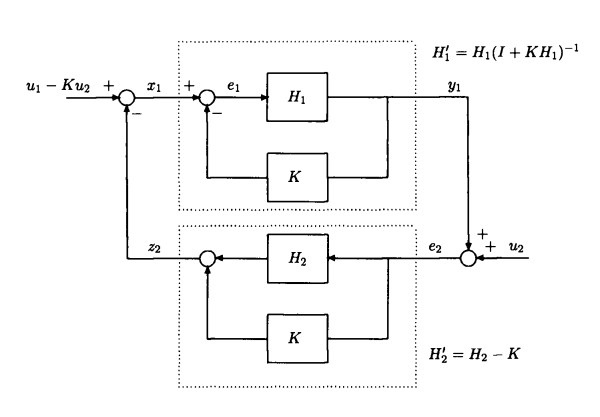
\includegraphics[width=\linewidth]{Images/nonlinear/ipopstability/sk.png}
    \caption{The feedback system $S_k$}
    \label{fig:feedback_sk}
\end{figure}


\begin{definition}[Type I Loop Transformation]
Consider the feedback system $S$ of Figure~\ref{fig:feedback}.  
Let $H_1, H_2, K$ and $(I+KH_1)^{-1}$ be causal maps from $X_e$ into $X$, and assume that $K$ is linear.  

A loop transformation of Type I is defined to be the modified system, denoted $S_K$, formed by the feedback interconnection of the subsystems
\[
H_1' = H_1 (I+KH_1)^{-1}, \qquad H_2' = H_2 - K,
\]
with inputs
\[
u_1' = u_1 - Ku_2, \qquad u_2' = u_2,
\]
as shown in Figure~\ref{fig:feedback_sk}.  

The closed-loop relations of $S_K$ will be denoted $E_K$ and $F_K$.
\end{definition}

\begin{theorem}
Consider the system $S$ of Figure~\ref{fig:feedback} and let $S_K$ be the modified system obtained after a Type I loop transformation. Assume $K$ and $(I+KH_1)^{-1}: X \to X$. Then:
\begin{enumerate}
    \item The system $S$ is stable if and only if the system $S_K$ is stable.
\end{enumerate}
\end{theorem}

\begin{figure}[h!]
\centering
\begin{tikzpicture}[auto, node distance=1.5cm, thick, >=latex]
  % Nodes
  \node (u1) {$u_1$};
  \node[draw, rectangle, minimum width=1.5cm, minimum height=1cm, right=of u1] (Minv) {$M^{-1}$};
  \node[circle, draw, minimum size=8mm, right=1.8cm of Minv] (sum1) {};
  \node[draw, rectangle, minimum width=1.5cm, minimum height=1cm, right=2.1cm of sum1] (M) {$M$};
  \node[draw, rectangle, minimum width=1.5cm, minimum height=1cm, right=of M] (H1) {$H_1$};

  \node[draw, rectangle, minimum width=1.5cm, minimum height=1cm, below=2.2cm of sum1] (Minv2) {$M^{-1}$};
  \node[draw, rectangle, minimum width=1.5cm, minimum height=1cm, right=of Minv2] (H2) {$H_2$};
  \node[circle, draw, minimum size=8mm, right=2.1cm of H2] (sum2) {};
  \node[right=2.1cm of sum2] (u2) {$u_2$};

  % Connections - Top path
  \draw[->] (u1) -- (Minv);
  \draw[->] (Minv) -- node[above] {$u_1'$} (sum1); 
  \draw[->] (sum1) -- node[above] {$x_1$} (M);
  \draw[->] (M) -- node[above] {$e_1$} (H1);

  % Feedback from H1 output to sum2 (no separate y1 node)
  \draw[->] (H1) |- ++(0,-2) -| (sum2);

  % Bottom path
  \draw[->] (Minv2) -- ++(0,2.2cm) -| node[pos=0.25,left] {$z_2$} (sum1);  
  \draw[->] (H2) -- node[below] {$y_2$} (Minv2);
  \draw[->] (sum2) -- node[below] {$e_2$} (H2);
  \draw[->] (u2) -- (sum2);

  % Labels on connections
  \node at ([xshift=1.3cm]sum1) [above] {};
  \node at ([xshift=1.15cm]M) [above] {};
  \node at ([xshift=0cm,yshift=-1.2cm]sum1) [left] {};
  \node at ([xshift=1.3cm]Minv2) [below] {};
  \node at ([xshift=1.3cm]H2) [below] {};

  % Signs
  \node at (sum1.center) {$+$};
  \node at ([xshift=-5pt, yshift=-7.5pt]sum1.center) {$-$};
  \node at (sum2.center) {$+$};
  \node at ([xshift=7.5pt, yshift=-5pt]sum2.center) {$+$};

\end{tikzpicture}
\caption{The Feedback System $S_M$}
\label{fig:feedback_sm}
\end{figure}


\begin{definition}[Type II Loop Transformation]
Consider the feedback system $S$ of Figure~\ref{fig:feedback}.  
Let $H_1, H_2$ be causal maps of $X_e$ into $X$, and let $M$ be a causal linear operator satisfying:  

\begin{enumerate}
    \item $M: X \to X$,  
    \item $M^{-1}: X \to X$ with $MM^{-1}=I$, and $M^{-1}$ is causal,  
    \item both $M$ and $M^{-1}$ have finite gain.  
\end{enumerate}

A Type II loop transformation is defined to be the modified system $S_M$, formed by the feedback interconnection of the subsystems
\[
H_1' = H_1 M, \qquad H_2' = M^{-1} H_2,
\]
with inputs
\[
u_1' = M^{-1}u_1, \qquad u_2' = u_2,
\]
as shown in Figure~\ref{fig:feedback_sm}.  

The closed-loop relations of this modified system will be denoted $E_M$ and $F_M$.
\end{definition}

\begin{theorem}
Consider the system $S$ of Figure~\ref{fig:feedback} and let $S_M$ be the modified system obtained after a Type II loop transformation. Then:
\[
S \text{ is stable } \iff S_M \text{ is stable.}
\]
\end{theorem}

%------------------------------------------------
\section{The Circle Criterion}\index{Circle Criterion}

Historically, one of the first applications of the small gain theorem was the celebrated \emph{circle criterion}, which analyzes the $\mathcal{L}_2$ stability of nonlinear feedback systems.  

\begin{definition}[Sector Condition]
A function $\phi:\mathbb{R}^+\times\mathbb{R}\to\mathbb{R}$ belongs to the sector $[\alpha,\beta]$ with $\alpha<\beta$ if
\begin{equation}
    \alpha x^2 \leq x\phi(t,x) \leq \beta x^2, \quad \forall t\geq 0,\ \forall x\in\mathbb{R}.
\end{equation}
\end{definition}

The Nyquist stability criterion provides necessary and sufficient conditions for the closed-loop stability of LTI systems with transfer function
\[
    G(s) = g(s) + \frac{n(s)}{d(s)},
\]
where $g(s)$ is stable, $n(s),d(s)$ are polynomials, and all zeros of $d(s)$ lie in the closed right-half plane. The number of open right-half plane zeros of $d(s)$ is denoted $v$.  

\begin{proposition}[Nyquist Criterion]
Consider the feedback of $H_1$ (with transfer function $d(s)$) and a constant gain $K$. The system is $\mathcal{L}_p$-stable ($1<p<\infty$) iff the Nyquist plot of $G(j\omega)$ avoids the point $(-1/K,0)$ and encircles it exactly $v$ times counterclockwise as $\omega$ goes from $-\infty$ to $\infty$.
\end{proposition}

\begin{theorem}[Circle Criterion]
Consider the feedback interconnection of an LTI system $H_1$ with transfer function $G(s)$ (satisfying the above assumptions) and a nonlinearity $\phi$ in the sector $[\alpha,\beta]$. The closed-loop system is $\mathcal{L}_2$-stable if one of the following holds:
\begin{enumerate}[(a)]
    \item If $0 < \alpha < \beta$: the Nyquist plot of $\tfrac{n(s)}{d(s)}$ avoids the \emph{critical circle} $C'$ (centered on the real axis and passing through $(-1/\alpha,0)$ and $(-1/\beta,0)$) and encircles it $v$ times counterclockwise.
    \item If $0=\alpha<\beta$: $G(s)$ has no right-half plane poles and the Nyquist plot lies to the right of the vertical line $\Re(z) = -1/\beta$.
    \item If $\alpha<0<\beta$: $G(s)$ has no poles in the closed right-half plane and the Nyquist plot lies entirely inside the circle $C'$.
\end{enumerate}
\end{theorem}

%------------------------------------------------
\begin{figure}[h]
\centering
\begin{tikzpicture}[scale=1.2]
    % Axes
    \draw[->] (-3.5,0) -- (1,0) node[right] {$\Re$};
    \draw[->] (0,-2) -- (0,2) node[above] {$\Im$};

    % Points on real axis (-1/alpha, 0) and (-1/beta, 0)
    \coordinate (A) at (-3,0); % Example: -1/alpha
    \coordinate (B) at (-1,0); % Example: -1/beta

    % Circle through A and B centered on real axis
    \path (A) -- (B) coordinate[midway] (M);
    \draw[dashed] (M) circle [x radius=1, y radius=1];

    % Mark points
    \fill (A) circle (1.5pt) node[below] {$-\tfrac{1}{\alpha}$};
    \fill (B) circle (1.5pt) node[below] {$-\tfrac{1}{\beta}$};
    \fill (M) circle (1.5pt) node[below,yshift=-2pt] {center};

    % Nyquist path (schematic curve)
    \draw[thick,blue,->,>=stealth] (-2.5,-1.2) .. controls (-2,0.8) and (-1.5,-0.8) .. (-0.5,1);

    % Labels
    \node at (-2,1.5) {$C'$: critical circle};
    \node[blue] at (-0.8,1.2) {Nyquist plot};
\end{tikzpicture}
\caption{The critical circle $C'$ in the Nyquist plane, passing through $(-1/\alpha,0)$ and $(-1/\beta,0)$.}
\end{figure}
